\documentclass{beamer}
\usefonttheme{professionalfonts}
\RequirePackage{thesis-slides}



\begin{document}
\hspace*{-1.2cm}
\begin{frame}[plain]
\titlepage % Print the title page as the first slide
\end{frame}

\section{Introduction}
\begin{frame}{Why do we study Machine Learning theoretically?}
  \structure{Machine learning} builds a model for machines to learn from data without explicit instruction.
  \pause
  \vfill

  \begin{columns}
    \column{0.4\textwidth}
      \texttt{DALL$\cdot$E 2}~{\cite{ramesh2022hierarchical}} \\
      ``\emph{Two  Formula 1 cars  racing under the Pisa tower, digital art}''
    \column{0.6\textwidth}
      \includegraphics[width=0.8\textwidth]{figures/dalle.png}
  \end{columns}
  \pause
  \vfill

  \begin{alertblock}{Theory lacks!}
    Many practical ``recipes'' but far from full comprehension.
  \end{alertblock}

  \note[item]{
    The Digital era has given us a tremendous amount of data, much more of what we humans can process.
  }
  \note[item]{
    DALLE is an example of a generative model for images. An example of the application of ML with success!
  }

  \note[item]{
    We need comprehension to not waste resources, design better models and algorithms, and have a description of what del model is doing (sensitive data).
  }
\end{frame}

\begin{frame}[fragile]
  \vspace{-5pt}
  \frametitle{Supervised Learning}
  \begin{block}{What is it?}
    Learn how to accomplish a task, given some solved samples.
  \end{block}
  \vspace{-25pt}
  \pause
  \begin{columns}[t]
    \column{0.33\textwidth}
      \begin{center}
        \structure{Data samples} \\
        \begin{columns}
          \column{0.5\textwidth}
            \hfill
            \visible<2->{\includegraphics[width=0.8\textwidth]{figures/animales/cat1.jpg}}
          \column{0.5\textwidth}
            Cat
        \end{columns}
        \begin{columns}
          \column{0.5\textwidth}
            \hfill
            \visible<2->{\includegraphics[width=0.8\textwidth]{figures/animales/dog1.jpg}}
          \column{0.5\textwidth}
            Dog
        \end{columns}
        $\vdots$\\
        \begin{columns}
          \column{0.5\textwidth}
            \hfill
            \visible<2->{\includegraphics[width=0.8\textwidth]{figures/animales/cat3.jpg}}
          \column{0.5\textwidth}
            Cat
        \end{columns}
      \end{center}
    \pause

    \column{0.33\textwidth}
      \begin{center}
        \structure{Model Architecture} \\
        \vspace{3pt}
        \visible<3->{
        \begin{tikzpicture}
          % \filldraw[blue, thick, fill=blue!50] (-1,1.75) -- (-0.5,1.25) -- (-0.5,0.75) -- (-1,0.25) -- cycle;
          % \draw[dotted] (-1,1.75) -- (0,1.35);
          % \draw[dotted] (-0.5,1.25) -- (0,1.15);
          % \draw[dotted] (-0.5,0.75) -- (0,0.85);
          % \draw[dotted] (-1,0.25) -- (0,0.65);
          % \draw[draw=black, thick, rounded corners] (0,0) rectangle ++ (1,2);
          % \node[label={[rotate=-90]:parameters}] at (0.45,0.9) {};
          % \draw[->] (1,1) -- (1.5, 1) node[right] {Answer};
          \node[inner sep=0pt] at (0,1.8) {\includegraphics[width=.5\textwidth]{figures/animales/dog2.jpg}};
          \draw[->, thick] (0,1)--(0,.5);
          \filldraw[draw=black, fill=black!10,thick, rounded corners] (-1.2,0.5) rectangle ++ (2.2,-1.5);
          \draw[->, thick] (0,-1.)--(0,-1.5);
          \node[inner sep=0pt] at (0,-1.8) {Dog!};
          % \node[inner sep=0pt] at (0,-0.25) {Parametrized Model};
          \node[label={[align=center]Parametrized\\Model}] at (-0.1,-1.) {};
        \end{tikzpicture}
        }
      \end{center}
    \pause
    \column{0.33\textwidth}
      \begin{center}
        \structure{Algorithm} \\
        \vspace{10pt}
        \visible<4->{\includegraphics[width=0.6\textwidth]{figures/algorithm-icon.png}}
        Optimize parameters\\
        based on samples.
      \end{center}
  \end{columns}
  \pause
  \vfill

  \begin{alertblock}{Learning \(\neq\) Memorization}
    The model should be able to generalize
  \end{alertblock}
\end{frame}

\begin{frame}
  \frametitle{Neural Networks}
  \begin{columns}
    \column{0.2\textwidth}
      \hspace{-15pt}
      \includegraphics[width=1.5\textwidth]{figures/animales/cat2.jpg}
      
    \column{0.65\textwidth}
      \hfill
      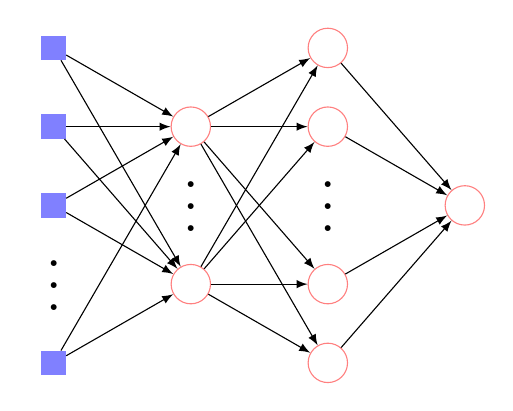
\begin{tikzpicture}[x=.87cm, y=1.cm, >=latex]
        \tikzset{
  inputnode/.style={
    rectangle,
    draw,
    minimum size=.3cm
  },
  every neuron/.style={
    circle,
    draw,
    minimum size=.5cm
  },
  neuron missing/.style={
    draw=none, 
    fill=none, %<- added
    scale=2,
    text height=0.333cm,
    execute at begin node=\color{black}$\vdots$
  }
}

\foreach \m [count=\y] in {1,2,3,missing,4} %<- removed "/\l" here 
  \node [fill=black,inputnode/.try, neuron \m/.try,blue!50] (input-\m) at (0,2.5-\y) {};
% added "fill=green" in the line above

\foreach \m [count=\y] in {1,missing,2}
  \node [every neuron/.try, neuron \m/.try,red!50] (hiddenone-\m) at (2,1.5-\y) {};

\foreach \m [count=\y] in {1,2,missing,3,4}
  \node [every neuron/.try, neuron \m/.try,red!50] (hiddentwo-\m) at (4,2.5-\y) {};

\foreach \m [count=\y] in {1}
  \node [every neuron/.try, neuron \m/.try,red!50] (output-\m) at (6,.5-\y) {};

% \foreach \l [count=\i] in {1,n}
%   \draw [->] (output-\i) -- ++(1,0)
%    node [above, midway] {$a_\l$};

\foreach \i in {1,...,4}
  \foreach \j in {1,...,2}
   \draw [->] (input-\i) -- (hiddenone-\j);

\foreach \i in {1,...,2}
  \foreach \j in {1,...,4}
    \draw [->] (hiddenone-\i) -- (hiddentwo-\j);

\foreach \i in {1,...,4}
  \foreach \j in {1}
    \draw [->] (hiddentwo-\i) -- (output-\j);

% \foreach \l [count=\x from 0] in {Eingangs-, Ausgangs-}
%   \node [align=center, above] at (\x*4,2) {\l \\ Neuronen};
      \end{tikzpicture}
    \column{0.15\textwidth}
      $\longrightarrow$ Cat!
  \end{columns}
  \begin{columns}
  \column{0.5\textwidth}
    \vspace{-30pt}

    \begin{center}
      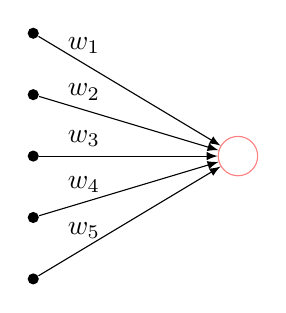
\begin{tikzpicture}[x=1.3cm, y=.78cm, >=latex]
      \tikzset{
  inputnode/.style={
    rectangle,
    draw,
  },
  every neuron/.style={
    circle,
    draw,
    minimum size=.5cm
  },
  neuron missing/.style={
    draw=none, 
    fill=none, %<- added
    scale=2,
    text height=0.333cm,
    execute at begin node=\color{black}$\vdots$
  }
}

\foreach \m [count=\y] in {1,2,3,4,5} %<- removed "/\l" here 
  \node [circle,fill,inner sep=0.05cm] (input-\m) at (0,2.5-\y) {};
% added "fill=green" in the line above

\foreach \m [count=\y] in {1}
  \node [every neuron/.try, neuron \m/.try,red!50] (output-\m) at (2,.5-\y) {};

% \foreach \l [count=\i] in {1,2,3,d}
%   \path (input-\i) -- ++(-1,0)
%    node [midway] {$x_\l$};

% \foreach \l [count=\i] in {1}
%   \path (output-\i) -- ++(1.3,0)
%     node [near end] {$\sigma\left(\vec{v}\cdot\vec{x}+b\right)$};

\foreach \i in {1,...,5}
  \foreach \j in {1}
    \draw [->] (input-\i) -- (output-\j);

\foreach \l [count=\i] in {1,2,3,4,5}
  \foreach \j in {1}
    \path (input-\i) -- (output-\j)
      node [above,near start] {$w_\l$};

% \foreach \l [count=\x from 0] in {Eingangs-, Ausgangs-}
%   \node [align=center, above] at (\x*4,2) {\l \\ Neuronen};
      \end{tikzpicture}
    \end{center}
  \column{0.5\textwidth}

  \pause
  \begin{exampleblock}{Why are they popular?}
    % \begin{columns}
    %   \column{0.5\textwidth}
          \begin{itemize}
            \item Universal approximator
            \item Good at generalizing
        %   \end{itemize}
        % \column{0.5\textwidth}
        %   \begin{itemize}
            \item Efficient algorithms
            % \item Highly versatile
          \end{itemize}
    % \end{columns}
  \end{exampleblock}
  \end{columns}
\end{frame}

\begin{frame}{Outline}
  \begin{exampleblock}{Why are we studying machine learning as physicist?}
    High dimensional system are in the realm of statistical physics!
  \end{exampleblock}
  \vfill
  \pause

  \structure{What are we going to present?}
  \begin{itemize}
    \item The particular setting of our study;
    \item Derive the equations for the dynamic;
    \item Study the overparametrization through learning times;
    \item Stochastic corrections to the equations.
  \end{itemize}
\end{frame}

\section{The setting}
\begin{frame}
\frametitle{The model architecture}
Goal: learn a \emph{predictor} \(\hat{f}\) given some samples \((\vec{x},y)\in\Real^{d+1}\).
\vfill
\begin{columns}
  \column{0.4\textwidth}
    \structure{Soft Committee Machine}
    \vspace{1.5pt}

    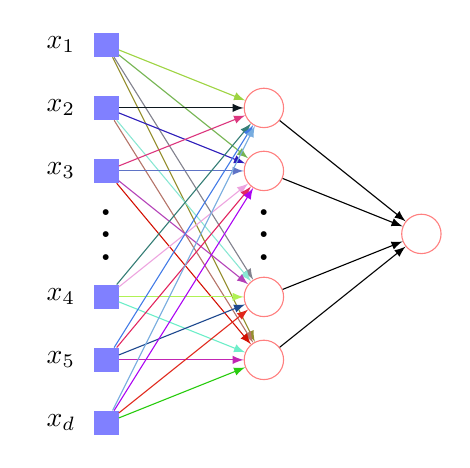
\begin{tikzpicture}[x=1cm, y=.8cm, >=latex]
      \tikzset{
  inputnode/.style={
    rectangle,
    draw,
    minimum size=.3cm
  },
  every neuron/.style={
    circle,
    draw,
    minimum size=.5cm
  },
  neuron missing/.style={
    draw=none, 
    fill=none, %<- added
    scale=2,
    text height=0.333cm,
    execute at begin node=\color{black}$\vdots$
  }
}

\pgfmathparse{rnd}
\xdefinecolor{MyColor}{rgb}{\pgfmathresult, 1.0, 1.0}

\foreach \m [count=\y] in {1,2,3,missing,4,5,6} %<- removed "/\l" here 
  \node [fill=black,inputnode/.try, neuron \m/.try,blue!50] (input-\m) at (0,2.5-\y) {};
% added "fill=green" in the line above

\foreach \m [count=\y] in {1,2,missing,3,4}
  \node [every neuron/.try, neuron \m/.try,red!50] (hidden-\m) at (2,1.5-\y) {};

\foreach \m [count=\y] in {1}
  \node [every neuron/.try, neuron \m/.try,red!50] (output-\m) at (4,-.5-\y) {};

\foreach \l [count=\i] in {1,2,3,4,5,d}
  \path (input-\i) -- ++(-1,0)
   node [midway] {$x_\l$};

% \foreach \l [count=\i] in {1,n}
%   \draw [->] (output-\i) -- ++(1,0)
%    node [above, midway] {$a_\l$};

\foreach \i in {1,...,6}
  \foreach \j in {1,...,4} {
    \edef\R{\pdfuniformdeviate 255}
    \edef\G{\pdfuniformdeviate 255}
    \edef\B{\pdfuniformdeviate 255}
    \xdefinecolor{MyColor}{RGB}{\R,\G,\B}
    \draw [->,MyColor] (input-\i) -- (hidden-\j);
  }


\foreach \i in {1,...,4}
  \foreach \j in {1}
    \draw [->] (hidden-\i) -- (output-\j);

% \foreach \l [count=\x from 0] in {Eingangs-, Ausgangs-}
%   \node [align=center, above] at (\x*4,2) {\l \\ Neuronen};
    \end{tikzpicture}
  \column{0.6\textwidth}
    \[\hat{f}\colon \Real^d\to\Real\]
    \[\hat{f}{(\vec{x})} = \frac{1}{p}\sum_{j=1}^{p} \act{\left(\frac{\vec{w}_j \cdot \vec{x}}{\sqrt{d}}\right)}\]
    \vspace{30pt}

    \begin{center}The network \emph{parameters} are\end{center} 
    \[\vec{w}_j \coloneqq [\W]_j \in \Real^d\]
    \[\W \in \Real^p\times\Real^d\]
\end{columns}
\note[item]{Must define \(d, p, \act\). They are \textbf{meta}parameters}
\note[item]{Stress the fact that the \emph{hat} is for the predictor.}
\note[item]{Just one real output, but it's not a problem.}
\note[item]{Fixed weights in the second layer, can be done with more but it's just complicated.
            More parameters, no gain.}
\note[item]{
  Stress out that here we are doing regression and not classification. The output is continuous!
}
\end{frame}

\begin{frame}
  \frametitle{Data samples}
  The input samples are \emph{indipendent normal distributed}
  \[
    \vec{x} \sim \gauss{(0,\I_d)}.
  \]
  \pause

  The output \(y\) is generated by a \emph{teacher} model with the same architecture
  \[
    f{(\vec{x})} = \frac{1}{k}\sum_{r=1}^{k} \act{\left(\frac{\vec{w}^*_r \cdot \vec{x}}{\sqrt{d}}\right)}
    \quad\text{where}\quad \vec{w}^*_r \coloneqq [\W^*]_r \in \Real^d. 
  \]
  \pause

  We overlap some noise to the \(y\) label
  \[
    y = f{(\vec{x}) + \sqrt{\Delta}\xi}\quad\text{with } \xi \sim \gauss{(0,1)}
  \]
  \note[item]{
    We use Gaussians, but it's not mandatory. It has been done in the past \cite{refinetti2022dynamics}
  }
  \note[item]{
    \emph{Teacher-student setting}: the student knows anything about the architecture of the teacher.
    He observes only pairs. It's just a convenient way of writing a generative model that gives us control on the learning.
  }
  \note[item]{
    The teacher has \(k\le p\) as a realizability condition
  }
  \note[item]{
    Teacher has not the hat and the weights matrix has the asterisk
  }
  \note[item]{
    Must say \(\Delta\) is not a parameter of the network, but just a parameter of our theoretical model.
  }
\end{frame}

\begin{frame}
  \frametitle{Measuring the goodness}
  The \emph{loss function} measures distance in output spaces
  \[
    \only<1>{\loss\colon \Real\times\Real\to\Real^+}
    \only<2->{\loss\colon \Real\times\Real\to\Real^+ \qquad \loss{(y_1,y_2)}=\frac12 (y_1-y_2)^2}
  \]
  \pause

  The goodness of the \emph{predictor} over a sample \((\vec{x}_s,y_s)\) is 
  \[
    \loss{\left(\hat{f}{(\vec{x}_s)},y_s\right)}
  \]
  \pause

  The global performance instead
  \[
    \risk_\text{theo} 
    %= \E_{\vec{x}\sim\gauss{(0,\I_d)}}{\left[\loss{\left(f{\left(\vec{x}\right)},\hat{f}{\left(\vec{x}\right)}\right)}\right]}=
    =\frac{1}{2}\E_{\vec{x}\sim\gauss{(0,\I_d)}}{\left[\left(f{\left(\vec{x}\right)}-\hat{f}{\left(\vec{x}\right)}\right)^2\right]}
  \]
  \note[item]{
    The loss function is an important choice and really depends on the data used.
    Since we are working in a continuous setting this is the easiest choice.
    Moreover, it will lead to known models in the future (phase retrieval)
  }
  \note[item]{
    We have access to the theoretical risk just because we know both the distribution of \(\vec{x}\) and the
    generative model (teacher). We don't use it for the training, otherwise, we are not studying the realistic dynamics.
  }
  \note[item]{
    The risk is called theoretical because there is also the empirical one, on the sample one really knows, but it's not the case here.
  }
\end{frame}

\begin{frame}
  \frametitle{The algorithm}
  \begin{block}{Optimization}
    The best possible predictor has parameters
    \[
      \W_\text{best} \in \argmin_{\W}{\risk_\text{theo}}
    \]
  \end{block}
  \pause

  The algorithm we use is \emph{one-pass stochastic gradient descent}:
  \begin{enumerate}
    \item Sample a vector \(\vec{x}^\nu\) and generate \(y^\nu\) using the teacher.
    \item For every \(j\in[1,p]\)
          \[\w^{\nu+1}_j = \w^{\nu}_j - \gamma \nabla_{\w_j}\left(\loss\left(y^\nu,\hat{f}{\left(\vec{x}^\nu\right)}\right)\right)\]
  \end{enumerate}
  \pause

  \vspace{-15pt}
  \begin{alertblock}{Open question}
    The loss function is not convex, but the algorithm converges to nearly optimal solution
  \end{alertblock}

  \note[item]{
    Of course, the \(\argmin\) is not unique, but it's not important!
  }
  \note[item]{
    \(\nu\) is the index that indicates the number of samples used.
  }
  \note[item]{
    The formula is the updated rule of the weights.
  }
  \note[item]{
    \(\gamma\) is the \emph{learning rate}. It's an \textbf{hyper}parameter, a property only of the algorithm. 
    It affects the dynamics and the final state, but it's not something that the predictor knows.
  }
  \note[item]{
    If someone among you has experience in applying machine learning maybe it's used to \emph{full batch gradient descent} or
    \emph{stochastic gradient descent}, but also this algorithm is use.
  }
  \note[item]{
    Let's note that the training dynamics it's a discrete stochastic process in the space of the student weights matrix.
  }
\end{frame}

\section{Sufficient dynamic}
\begin{frame}
  \frametitle{Local fields}
  \begin{block}{Goal}
    Describe the training dynamic with some \emph{sufficient statics} of the weights
  \end{block}
  \pause
  \vfill

  % \begin{columns}
  %   \column{0.5\textwidth}
  %     \structure{Change of variables}
  %     \includegraphics[width=\textwidth]{example-image-duck}
  %   \column{0.5\textwidth}
    \[
      \vec{\lf} = \frac{\W\vec{x}}{\sqrt{{d}}}\quad
      \vec{\lf}^{*} = \frac{\W^{*}\vec{x}}{\sqrt{{d}}}
    \]
    \[\begin{split}
        \hat{f}{(\vec{x})} \rightarrow& \hat{f}{(\vec{\lf})} = \frac{1}{p}\sum_{j=1}^{p} \act{\left(\lf_j\right)} \\
        f{(\vec{x})} \rightarrow& f{(\vec{\lf}^*)} = \frac{1}{k}\sum_{r=1}^{k} \act{\left(\lf^*_k\right)}
    \end{split}\]

  % \end{columns}
  \note[item]{
    I want to do all the steps of this derivation (no calculations) to emphatize how this is 
  }
  \note[item]{
    The \(\lf\)s are called \emph{local fields} and are microscopic variables.
    They are correlated normal distributions, their scale is around 1 independently of \(d\). We see this in the next slides
  }
\end{frame}

\begin{frame}
  \frametitle{Order parameters}
  \(\vec{\lf},\vec{\lf}^*\) are normal random variables with 0 mean and covariance
  \[
    \frac{1}{d}\left(\begin{array}{cc}\W\W^\top &  \W\W^{*\top}\\ \W^{*}\W^\top & \W^*\W^{*\top}\end{array}\right) =
    \left(\begin{array}{cc}\Q & \M \\ \M^{\top} & \P \end{array}\right) =
    \vec{\Omega} \in \Real^{p+k}\times\Real^{p+k}
  \]
  \(\vec{\Omega}\) is the \emph{overlapping matrices};\\
  \(\Q,\M,\P\) are the \emph{order parameters}
  \pause 

  \vfill
  \(\vec{\Omega}\) is the sufficient statistic we use for describing the process
  \[\begin{split}
    \risk_\text{theo} &= \frac{1}{2}\E_{\vec{x}\sim\gauss{(0,\I_d)}}{\left[\left(f{\left(\vec{x}\right)}-\hat{f}{\left(\vec{x}\right)}\right)^2\right]} \\
                      &= \frac12\E_{\vec{\lf},\vec{\lf^* \sim \gauss{(0,\vec{\Omega})}}}
                              {\left[\left(f{(\vec{\lf}^*)} - f{(\vec{\lf})}\right)^2\right]} = \risk{(\vec{\Omega})}
  \end{split}\]
  \note[item]{
    The variance allows us to define the \emph{order parameters}. These are the \emph{macroscopic variable} of the system
    because they are not dependent on \(d\) order of magnitude.
  }
  \note[item]{
    They are sufficient statics because \(\Omega\) is enough for defining the distribution of the local fields.
  }
  \note[item]{
    Key fact: The expected value is now low dimensional! This is exaclty what we wanted!
  }
  \note[item]{
    \textbf{Ising analogy}: order parameters are \emph{magnetization}, risk is the \emph{hamiltonian}.
  }
\end{frame}

\begin{frame}[fragile]
  \frametitle{Update rule for order parameters}
  \[
    \left[\M^{\nu+1}\right]_{jr} = \frac{\w^{\nu+1}_j \w^{*\top}_r}{d}
    = \cdots = \left[\M^{\nu}\right]_{jr} + \frac{1}{d} \psi_{jr}{(\vec{\lf}^\nu,\vec{\lf}^{*\nu})}
  \]
  \pause
  \[
    \left[\Q^{\nu+1}\right]_{jl} 
    = \left[\Q^{\nu}\right]_{jl} + \frac{1}{d}\varphi_{jl}{(\vec{\lf}^\nu,\vec{\lf}^{*\nu})}
    \qquad \P\text{ is constant}
  \]
  \pause

  \begin{block}{Overlapping matrix dynamic}
    \[\left\{\vec{\Omega}^\nu \in \Real^{(p+k)\times(p+k)}|\nu\in\Natural\right\}\]
    \[
      \begin{tikzcd}
      \vec{\Omega}^0 \arrow[r,"\text{sample}"] \arrow[d] & \vec{\lf}^1,\vec{\lf}^{*1} \arrow[r,"\text{update}"] & \vec{\Omega}^1 \arrow[d] \arrow[r,dash,dotted] & \vec{\lf}^\nu,\vec{\lf}^{*\nu} \arrow[r,"\text{update}"] & \vec{\Omega}^\nu \arrow[d]\\
      \risk^0 & {} & \risk^1 & {} & \risk^\nu
      \end{tikzcd}
    \]
  \end{block}

  \note[item]{
    We can use the update rule on weights to compute an update rule on parameters.
    It's not obvious that it's possible to have an update rule on order parameters, but we did.
  }
  \note[item]{
    We can fully describe the learning process by looking at the dynamic of matrix \(\vec{\Omega}\).
    The risk is just a function of \(\Omega\), so there is no need to keep all the weights to monitor learning (we gain a lot in term of storage of information).
    Nevertheless, we will use the weights matrix properties in simulations or for initialization, but the theoretical study can be restricted to this matrix!
  }
\end{frame}

\begin{frame}
  \frametitle{High dimensional limit}
  We take the limit \(d\to+\infty\)
  \[
    \frac{\M^{\nu+1} - \M^{\nu}}{\frac1d} = \vec{\psi}{(\vec{\lf}^\nu,\vec{\lf}^{*\nu})}
    \qquad \delta t = \frac1d 
  \]
  \pause

  \begin{exampleblock}{Differential Equations of the process}
    \emph{Saad\&Solla equations} \cite{saad1995line}
    \begin{align*}
      \dod{\M{\left(t\right)}}{t} &=\E_{\vec{\lf},\vec{\lf^* \sim \gauss{(0,\vec{\Omega}{(t)})}}}{\left[\psi{(\vec{\lf}^\nu,\vec{\lf}^{*\nu})}\right]} \eqqcolon \Psi{\left(\vec{\Omega}\right)}\\
      \dod{\Q{\left(t\right)}}{t} &=\E_{\vec{\lf},\vec{\lf^* \sim \gauss{(0,\vec{\Omega}{(t)})}}}{\left[\phi{(\vec{\lf}^\nu,\vec{\lf}^{*\nu})}\right]} \eqqcolon \Phi{\left(\vec{\Omega}\right)},
    \end{align*}
    \vspace{-10pt}
    \begin{itemize}
      \item Discrete index is mapped to time with \(t=\frac{\nu}{d}\)
      \item The expected error between the two is given by \(\frac{1}{\sqrt{d}}\)
    \end{itemize}
  \end{exampleblock}

  \note[item]{
    LHS is the derivative of the order parameter matrix;
    RHS is less clear. The intuition is given by the CLT: the fluctuations are killed beacuse we are using a lot of indipendent gaussian.
    RHS concentrates to the mean and converges to the expected value of the expression.
    Again this depends only on the shape of the distribution of \(\lf\)s, so this expected value is function of just \(\vec{\Omega}\)
  }
  \note[item]{
    The differential equations depend on \(\gamma, p, k, \sigma\)
  }
  \note[item]{
    These equations are the fundamental result used in this work relay on.
    They give us a \emph{deterministic} dynamic for the evolution, starting from a stochastic process
  }
  \note[item]{
    There is a formal formulation of this fact given by \cite{goldt2019dynamics}. It's mathematically proved! 
  }
\end{frame}

\section{Results}
\begin{frame}
  \frametitle{Specilazing to activation function}
  Special choice of activation function
  \[
    \act{(x)} = x^2
  \]
  We used \emph{Isserlis' Theorem} for computing the expected values
  \pause
  \vfill
  Example of an equation:
  \[
    \dod{\M}{t} = \frac{2 \gamma}{p}\left[
        \left(\frac{\Tr{\P}}k - \frac{\Tr{\Q}}p\right)\M +
        2\left(\frac{\M\P}{k} - \frac{\Q\M}{p}\right)
    \right]
  \]
  \pause
  \vfill
  \begin{block}{Special case: \textbf{\emph{phase retrivial}}}
    \(k=p=1 \implies\)Many result in literature \\
    \(\M, \Q\) and \(\P\) are scalars.

  \end{block}

  \note[item] {
    We choose this instead of \(\erf\) because gives us simpler equations.
  }
\end{frame}

\begin{frame}{Expected dynamics of the risk}
  \begin{center}
    \begin{tikzpicture}[
      x=.7cm,
      y=.7cm
    ]
      \filldraw [fill=Background,draw opacity=0.] (0,0) rectangle (10.,9.);
\draw[black, ->, thick] (0,0) -- (10,0) node[below] {\(t\)};
\draw[black, ->, thick] (0,0) -- (0, 9) node[left] {\(\mathcal{R}\)};

\draw[
  line width=1.5mm,
  Red,
  looseness=1.1
] (0,8) to[out=0, in=180]
  (1.0,8) to[out=0, in=180]
  (2., 7) to[out=0, in=180] 
  (10, 7);

\draw[
  line width=1.mm,
  Blue,
  looseness=1.1
] (0,8) to[out=0, in=180]
  (1.0,8) to[out=0, in=180]
  (2., 7) to[out=0, in=180] 
  (4., 7) to[out=0, in=180]
  (5., 5) to[out=0, in=180]
  (10, 5);

\draw[
  line width=0.5mm,
  Green,
  looseness=1.1
] (0,8) to[out=0, in=180]
  (1.0,8) to[out=0, in=180]
  (2., 7) to[out=0, in=180] 
  (4., 7) to[out=0, in=180]
  (5., 5) to[out=0, in=180]
  (6., 5) to[out=0, in=180]
  (8., 1.5) to[out=0, in=180]
  (10., 1.5);

\node[right] at (1.5,7.55) {norm learning};
\node[left] at (4.5,6.) {linear learning};
\node[left] at (7.,3.25) {specialization};
    \end{tikzpicture}
  \end{center}
  
\end{frame}

\begin{frame}
  \frametitle{Comparsion simulation vs ODEs }
  % \begin{columns}
  %   \column{0.75\textwidth}
    \begin{center}
      \includegraphics[width=0.8\textwidth]{figures/simulation_examples_trajectory.pdf}
    \end{center}
  %   \column{0.4\textwidth}
  %     {}
  % \end{columns}
\end{frame}

\begin{frame}
  \frametitle{Spherical Constraint}
  Force the weights on the sphere to exclude norm learning
  \[
    \vec{w}^\nu_j, \vec{w}^*_r \in S^{d-1}{\left(\sqrt{d}\right)}\qquad
    \w^{\nu+1}_j =\frac{\w^{\nu}_j - \gamma \nabla_{\w_j}{\loss}}{\left\|\w^{\nu}_j - \gamma \nabla_{\w_j}{\loss}\right\|}\sqrt{d}
  \]
  \pause
  \vfill

  \begin{exampleblock}{New dynamic}
    \emph{Saad\&Solla Equations} for spehrical dynamics
    \[\begin{split}
      \dod{\left[\M{\left(t\right)}\right]_{jr}}{t} &= \Psi_{jr}{(\vec{\Omega})} - \frac{\left[\M{\left(t\right)}\right]_{jr}}{2}\Phi_{jj}{(\vec{\Omega})} \\
      \dod{\left[\Q{\left(t\right)}\right]_{jl}}{t} &= \Phi_{jl}{(\vec{\Omega})} - \frac{\left[\Q{\left(t\right)}\right]_{jl}}{2}\left(\Phi_{jj}{(\vec{\Omega})}+\Phi_{ll}{(\vec{\Omega})}\right)
    \end{split}\]
  \end{exampleblock}
\end{frame}

\begin{frame}
  \frametitle{Spherical Phase retrieval}
  \vspace{-10pt}
  \begin{center}
    \includegraphics[width=.74\textwidth]{figures/spherical/spr-example-d10000-zoom.pdf}
  \end{center}
    \vspace{-8pt}
    \[
      t^\text{(pr)}_e = \frac{\log\left[1+T(d-1)\right]}{2\left(4\gamma(1-6\gamma)-2\gamma^2\Delta\right)}
      \qquad
      \lim_{t\to\infty}\risk(t) = \frac{\gamma\Delta}{1-6\gamma}
    \]
\end{frame}

\begin{frame}
  \frametitle{Overparametrization gain}
  \begin{columns}
    \column{0.55\textwidth}
      \hspace{-7pt}
      \includegraphics[width=1.\textwidth]{figures/spherical/gamma_te-factor.pdf}
    \column{0.5\textwidth}
      \hfill It exists an optimal \(\gamma\) given \(p\)!\\
      \vspace{5pt}
      \hfill \(t_\text{opt} \coloneqq\) best exit time achievable
  \end{columns}
  \begin{columns}
    \column{0.55\textwidth}
      \[
        \frac{t_\text{opt}{(k)}}{\lim_{p\to+\infty}t_\text{opt}{(p)}} =
        \frac{\Delta k^2 + 4k + 8}{\Delta k^2 + 2k}
      \]
    \column{0.45\textwidth}
      \(\approx 6\) for gen. phase retrieval\\
      \(\approx 2\) for large \(k\)
  \end{columns}
\end{frame}

\section{Stochastich corrections}
\begin{frame}
  \frametitle{Stochastich corrections}
  Stick with phase retrieval.
  \begin{exampleblock}{Correction terms to \emph{Saad\&Solla Equations}}
    We introduce Brownian motion
    \[\begin{split}
      \dif m =& \Psi{(m,q)}\dif t + \frac{\vec{\sigma}_m{(m,q)}\cdot\dif \vec{W}}{d} \\
      \dif q =& \Phi{(m,q)}\dif t + \frac{\vec{\sigma}_q{(m,q)}\cdot\dif \vec{W}}{d} 
    \end{split}\]
  \end{exampleblock}
  \pause 

  \begin{itemize}
    \item Unconstrainted in accordance with \cite{arous2022high};
    \item Itô Calculus to force spherical dynamic.
  \end{itemize}
\end{frame}

\begin{frame}
  \frametitle{Stochastich correctionts to spherical phase retrieval}
  \begin{center}
    \includegraphics[width=.85\textwidth]{figures/sde/spr_final_zoom.pdf}
  \end{center}
\end{frame}

\section{Conclusion}
\begin{frame}
  \frametitle{Further Developments}
  \begin{itemize}
    \item Extend stochastic corrections to generic committee machine;
    \item Repeat the analysis for the specialization phase;
    \item Try to make the network deeper.
  \end{itemize}
  \vfill

  \begin{center}
    \visible<2->{\structure{\Huge Thank you for the attention!}}
  \end{center}
\end{frame}

\setbeamertemplate{page number in head/foot}{\phantom{0/0}}
\begin{frame}[noframenumbering, allowframebreaks]
  \frametitle{Bibliography}
  % \textbf{\structure{Bibliography}}
  \printbibliography
  \vspace{3cm}
\end{frame}

\begin{frame}
  \frametitle{Logarithm vs Polynomial}
  Fit for the unconstrained phase retrivial
  \begin{center}
    \includegraphics[width=1.05\textwidth]{figures/log_fit.pdf}
  \end{center}
\end{frame}

\end{document}
